\subsection{Desigualdade da soma de logaritmos}
\begin{frame}%[allowframebreaks]
  \frametitle{Desigualdade da soma de logaritmos}
  \begin{theorem}[desigualdade da soma de logaritmos]
  Dados $(a_1, \ldots, a_n)$ e $(b_1,\ldots,b_n)$, com $a_i \geq 0$ e $b_i \geq 0$, temos
        \begin{equation}
         \sum_{i=1}^n a_i \log \frac{a_i}{b_i} \geq \left( \sum_{i=1}^n a_i \right) \log \frac{\sum_{i=1}^n a_i}{\sum_{i=1}^n b_i}
        \end{equation}
  e teremos igualdade sse $a_i/b_i = c = \text{const.}$.
  \end{theorem}

  \begin{itemize}
  \item Relembrando: $0 \log 0 = 0$, $a \log a/0 = \infty$ para $a>0$, e $0 \log 0/0 =0$.
  \item A desigualdade da soma de logaritmos é utilizada para demonstrar algumas propriedades importantes.
  \end{itemize}
\end{frame}

\begin{frame}%[allowframebreaks]
  \frametitle{Desigualdade da soma de logaritmos}

  Considere $f(t) = t \log t = t (\ln t) (\log e)$, que é estritamente convexa, pois
  $f''(t) = 1/t \log e >0$, $\forall t > 0$.
  
  \begin{figure}[h!]
  \centering
  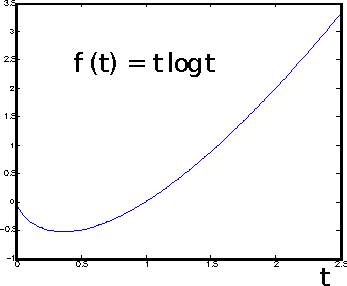
\includegraphics[width=0.4\textwidth]{images/tlogt.pdf}
  %\caption{.}
  \label{fig:tlogt}
  \end{figure}
\end{frame}

\begin{frame}[allowframebreaks]
  \frametitle{Desigualdade da soma de logaritmos}
  \begin{proof}
        \begin{itemize}
        \item Dada $f$ convexa, a desigualdade de Jensen diz que
          \begin{equation}
          \sum_i \alpha_i f(t_i) \geq f \left( \sum_i \alpha_i t_i \right) \text{ com } \alpha_i \geq 0 \text{ e } \sum_i \alpha_i = 1
          \end{equation}

        \item $f(x) = x \log x$ é estritamente convexa para $x>0$, já que 
                $f''(x)=\frac{1}{x} \log e > 0$ para $x>0$.

        \end{itemize}
        \proofbreak
        \begin{itemize}
        \item Vamos fazer $\alpha_i = \nicefrac{b_i}{\sum_{j=1}^n b_j}$ e $t_i = \nicefrac{a_i}{b_i}$, então teremos
        \begin{eqnarray}
        \sum_i \alpha_i f(t_i) &\geq& f \left( \sum_i \alpha_i t_i \right) \nonumber \\
        \sum_i \left( \frac{b_i}{\sum_j b_j} f \left( \frac{a_i}{b_i} \right) \right) &\geq&
                f \left( \sum_i \frac{b_i}{\sum_j b_j} \frac{a_i}{b_i} \right) \nonumber
        \end{eqnarray}
        \end{itemize}

   \proofbreak
   \vspace{-2ex}
   \begin{eqnarray}
        \sum_i \left( \frac{b_i}{\sum_j b_j} f \left( \frac{a_i}{b_i} \right) \right) &\geq&
                f \left( \sum_i \frac{b_i}{\sum_j b_j} \frac{a_i}{b_i} \right) \nonumber \\
        \frac{1}{\sum_j b_j} \sum_i \left( b_i \frac{a_i}{b_i} \log \frac{a_i}{b_i} \right) &\geq&
                \left( \sum_i \frac{a_i}{\sum_j b_j} \right) \log \sum_i \frac{a_i}{\sum_j b_j} \nonumber \\
        \sum_i a_i \log \frac{a_i}{b_i} &\geq& \left( \sum_i a_i \right) \log \sum_i \frac{a_i}{\sum_j b_j} \nonumber \\
        \sum_i a_i \log \frac{a_i}{b_i} &\geq& \sum_i a_i \log \frac{\sum_i a_i}{\sum_j b_j}
   \end{eqnarray}

  \end{proof}
\end{frame}


\subsection{Divergência é não negativa}
\begin{frame}%[allowframebreaks]
  \frametitle{Divergência é não negativa}
  A desigualdade da soma de logaritmos pode ser utilizada para mostrar que $D(p||q) \geq 0$.
  \begin{proof}
        \begin{eqnarray}
        D(p||q) &=& \sum_x p(x) \log \frac{p(x)}{q(x)} \nonumber \\
                &\geq& \left( \sum_x p(x) \right) \log \frac{\sum_x p(x)}{\sum_x q(x)} \nonumber \\
                &=& 1 \log \frac{1}{1} = 0
        \end{eqnarray}
  \end{proof}
\end{frame}

\subsection{Entropia Relativa é Convexa no Par}
\begin{frame}[allowframebreaks]
  \frametitle{A Entropia Relativa é Convexa no Par}
  \begin{theorem}
  Seja $(p_1, q_1)$ e $(p_2, q_2)$ dois pares de função massa probabilidade, então
    \begin{equation}
        D(\lambda p_1 + (1 - \lambda) p_2 || \lambda q_1 + (1- \lambda)q_2) \leq \lambda D(p_1 || q_1) + (1- \lambda) D(p_2 || q_2) ,
    \end{equation}
    para todo $0 \leq \lambda \leq 1$.
  \end{theorem}

  \framebreak

  \begin{proof}
  Pela definição da divergência de KL, temos
    \begin{multline}
    D(\lambda p_1 + (1 - \lambda) p_2 || \lambda q_1 + (1- \lambda)q_2) = \\
        \sum_x (\lambda p_1(x) + (1 - \lambda) p_2(x) ) \log \frac{\lambda p_1(x) + (1 - \lambda) p_2(x)}{\lambda q_1(x) + (1 - \lambda) q_2(x)}
    \end{multline}
    cada termo do somatório é da forma
    \begin{equation}
        ( \lambda p_1(x) + (1 - \lambda) p_2(x) ) \log \frac{\lambda p_1(x) + (1 - \lambda) p_2(x)}{\lambda q_1(x) + (1 - \lambda) q_2(x)} = \left( \sum_i a_i \right) \log \frac{\sum_i a_i}{\sum_i b_i}
    \end{equation}

  \proofbreak

  Utilizando a desigualdade da soma dos logaritmos 
  \begin{eqnarray}
  \left( \sum_i a_i \right) \log \frac{\sum_i a_i}{\sum_i b_i} &\leq&
        \sum_i a_i \log \frac{a_i}{b_i} \nonumber \\
        &=& a_1 \log \frac{a_1}{b_1} + a_2 \log \frac{a_2}{b_2} \nonumber \\
        &=& \lambda p_1(x) \log \frac{\lambda p_1(x)}{\lambda q_1(x)} + (1 - \lambda) p_2(x) \log \frac{(1 - \lambda) p_2(x)}{(1-\lambda) q_2(x)} \nonumber \\
        &=& \lambda D(p_1 || q_1) + (1 - \lambda) D(p_2 || q_2)
  \end{eqnarray}
  \end{proof}
\end{frame}
\note{
        \begin{itemize}
        \item Note que podemos fazer $q_1 = q_2$ e desta forma obteremos convexidade apenas em $p$.
        \item Este é o fundamento para o procedimento de minimização alternada, que
        é um caso especial do algoritmo de EM (maximização da esperança), 
        para o cálculo da função de taxa de distorção,
        e para o cálculo da função geral de capacidade de canal.
        \end{itemize}
}

\subsection{Concavidade da Entropia}
\begin{frame}[allowframebreaks]
  \frametitle{A Entropia é Concava}
  \begin{theorem}
  $H(p)$ é uma função concava de $p$.
  \end{theorem}

  \framebreak
  \begin{proof}
  \vspace{-4ex}
  \begin{eqnarray}
    H(p) &=& - \sum_i p_i \log p_i = - \sum_i p_i \log p_i  + \log \vert \mathcal{X} \vert - \log \vert \mathcal{X} \vert \nonumber \\
        &=& \log \vert \mathcal{X} \vert - \sum_i p_i \log p_i - \log \vert \mathcal{X} \vert \underbrace{\sum_i p_i}_{=1} \nonumber \\
        &=& \log \vert \mathcal{X} \vert - \sum_i \left( p_i \log p_i + p_i \log \vert \mathcal{X} \vert \right) \nonumber \\
        &=& \log \vert \mathcal{X} \vert - \sum_i p_i \left( \log p_i -  \log \nicefrac{1}{\vert \mathcal{X} \vert } \right) \nonumber \\
        &=& \underbrace{\log \vert \mathcal{X} \vert}_{\text{constante}} - \underbrace{D(p||u)}_{\text{convexo}}
  \end{eqnarray}
  onde $u$ é a distribuição uniforme.
  \end{proof}
\end{frame}
\note{
Podemos ver a entropia como a similaridade com a distribuição uniforme.
Quanto maior a entropia, mais próximo estaremos da distribuição uniforme.
}

\begin{frame}[allowframebreaks]
  \frametitle{Consequências para a Informação Mútua}
  Seja $(X,Y) \sim p(x,y) = p(x)p(y|x)$, a informação mútua $I(X;Y)$ é uma função côncava
  de $p(x)$ para $p(y|x)$ fixo e uma função convexa de $p(y|x)$ para $p(x)$ fixo.

  \framebreak
  \begin{proof}
    \begin{itemize} \item $I(X;Y)$ é uma função côncava de $p(x)$ para $p(y|x)$ fixo \end{itemize}
    \vspace{-2ex}
    \begin{eqnarray}
    I(X;Y) &=& D(p(x,y)||p(x)p(y)) \text{ (definição) } \nonumber \\
        &=& \sum_{x,y} p(x,y) \log \frac{p(x,y)}{p(x)p(y)} \text{ (definição) } \nonumber \\
        &=& \sum_{x,y} p(x)p(y|x) \log \frac{ p(x)p(y|x) }{p(x) \sum_x p(x) p(y|x)}
    \end{eqnarray}
    Se $p(y|x)$ é constante, então a informação mútua é função de $p(x)$
    \vspace{-1ex}
    \begin{equation}
    I_{p(x)} (X;Y) = \sum_{x,y} p(x) p(y|x) \log \frac{p(x) p(y|x)}{p(x) \sum_x p(x) p(y|x)}
    \end{equation}  

    \proofbreak
    
    \begin{equation}
    I_{p(x)} (X;Y) = \sum_{x,y} p(x) p(y|x) \log \frac{p(x) p(y|x)}{p(x) \sum_x p(x) p(y|x)}
    \end{equation}

    Utilizando a propriedade da convexidade da divergência de Kullback-Leibler
    \begin{equation}\label{eq-Imixpx}
    I_{\lambda p_1(x) + (1-\lambda)p_2(x)} (X;Y) \geq \lambda I_{p_1(x)} (X;Y) + (1-\lambda) I_{p_2(x)} (X;Y)
    \end{equation}
    então a informação mútua é uma função concava de $p(x)$ para $p(y|x)$ fixo.


    \proofbreak

    \begin{itemize} \item $I(X;Y)$ é uma função convexa de $p(y|x)$ para $p(x)$ fixo \end{itemize}
    Aplicamos a mesma ideia, porém agora consideraremos $p(x)$ fixo.
    \begin{equation}
    I_{p(y|x)} (X;Y) = \sum_{x,y} p(x) p(y|x) \log \frac{p(x) p(y|x)}{p(x) \sum_x p(x) p(y|x)}
    \end{equation}

    Utilizando a propriedade da convexidade da divergência de Kullback-Leibler
    \begin{equation}\label{eq-Imixpxy}
    I_{\lambda p_1(y|x) + (1-\lambda)p_2(y|x)} (X;Y) \leq \lambda I_{p_1(y|x)} (X;Y) + (1-\lambda) I_{p_2(y|x)} (X;Y)
    \end{equation}

  \end{proof}
\end{frame}
\note{
Estes resultados serão importantes para a capacidade de canal e vários outras
otimizações envolvendo informação mútua e distribuições.
}

\begin{frame}[allowframebreaks]
  \frametitle{Informação Mútua, Comunicação e Convexidade}

  Envio de informação por um canal ruidoso.
  \begin{figure}[h!]
  \centering
  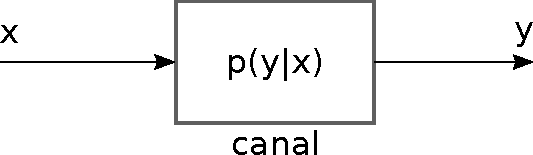
\includegraphics[width=0.5\textwidth]{images/canal_pyx.pdf}
  %\caption{.}
  \label{fig:3va-venn}
  \end{figure}

  \begin{itemize}
        \item Canal: processo ruidoso, para cada $x$ temos uma distribuição sobre os possíveis $y$ recebidos
        \item A taxa de informação transmitida de $X$ para $Y$, por utilização do canal,
        em unidades de bits, é $I(X;Y)$.
  \end{itemize}
\end{frame}
\note{
  \begin{itemize}
        \item Embaralhando $p(x)$ não pode diminuir (pode aumentar ou não alterar) 
        a transmissão de informação para um canal fixo, com relação à original mistura de taxas
        (ver Equação \ref{eq-Imixpx}).
        \item Embaralhando $p(y|x)$ para um canal ruidoso e uma fonte fixa, podemos apenas
        não aumentar (pode reduzir ou manter constante) a taxa de transmissão, em relação
        à original mistura de taxas (ver Equação \ref{eq-Imixpxy}).
  \end{itemize}
}


